% !TEX program = xelatex
\documentclass[aspectratio=169]{beamer}
\usepackage{amsmath}
\usepackage{amssymb}
\usepackage{graphicx}
\usepackage{tcolorbox}
\usepackage{booktabs}
\usepackage{colortbl}
\usepackage{xcolor}
\usepackage{tikz}
\usetikzlibrary{angles,quotes}
\usepackage[utf8]{inputenc}

% Custom colors
\definecolor{primary}{RGB}{41, 128, 185}
\definecolor{secondary}{RGB}{52, 152, 219}
\definecolor{accent}{RGB}{231, 76, 60}
\definecolor{lightgray}{RGB}{236, 240, 241}

% Theme customization
\usetheme{Madrid}
\usecolortheme{whale}
\setbeamercolor{structure}{fg=primary}
\setbeamercolor{background canvas}{bg=white}
\setbeamercolor{normal text}{fg=black}

% Title page info
\title{Pre-Calculus 11}
\subtitle{Chapter 8.1: Graphing Linear Inequalities with Two Variables}
\author{Created by Yi-Chen Lin}
\date{\today}

\begin{document}

% Title Page
\begin{frame}
    \titlepage
\end{frame}

% What is a Linear Inequality in Two Variables?
\begin{frame}{What is a Linear Inequality in Two Variables?}
    \begin{tcolorbox}[colback=lightgray,colframe=primary,title=Definition]
        \footnotesize
        A linear inequality in two variables is an inequality that can be written in the form $ax + by < c$, $ax + by \leq c$, $ax + by > c$, or $ax + by \geq c$.
        \begin{itemize}
            \item The solution is a region (half-plane) on the coordinate plane.
            \item The boundary is a straight line, which may be solid (included) or dotted (not included).
        \end{itemize}
    \end{tcolorbox}
    \vspace{0.5em}
    \textbf{Examples:}
    \begin{itemize}
        \item $y > 2x - 1$
        \item $3x + 2y \leq 6$
    \end{itemize}
\end{frame}

% Steps to Graph a Linear Inequality
\begin{frame}{How to Graph a Linear Inequality}
    \begin{tcolorbox}[colback=lightgray,colframe=primary,title=Step-by-Step Method]
        \footnotesize
        \begin{enumerate}
            \item \textcolor{accent}{\textbf{Graph the boundary line:}}
            \begin{itemize}
                \item Use a \textcolor{accent}{dotted line} for $<$ or $>$ (not included)
                \item Use a \textcolor{primary}{solid line} for $\leq$ or $\geq$ (included)
            \end{itemize}
            \item \textcolor{accent}{\textbf{Pick a test point}} not on the line (often $(0,0)$)
            \item Substitute the test point into the inequality:
            \begin{itemize}
                \item If it makes the inequality true, shade that side
                \item If false, shade the opposite side
            \end{itemize}
            \item \textcolor{accent}{\textbf{The shaded region is the solution set.}}
        \end{enumerate}
    \end{tcolorbox}
\end{frame}

% Example: Graph 3x + 2y > 6 (Step 1)
\begin{frame}{Example: Graph $3x + 2y > 6$}
    \begin{tcolorbox}[colback=secondary!10,colframe=primary,title=Step 1: Rearrange]
        \footnotesize
        \[
            3x + 2y > 6
        \]
        \[
            2y > -3x + 6
        \]
        \[
            y > -\frac{3}{2}x + 3
        \]
        \textcolor{accent}{Slope: $-\frac{3}{2}$, y-intercept: $3$}
    \end{tcolorbox}
\end{frame}

% Example: Graph 3x + 2y > 6 (Step 2)
\begin{frame}{Example: Graph $3x + 2y > 6$}
    \begin{tcolorbox}[colback=secondary!10,colframe=primary,title=Step 2: Graph the Line]
        \footnotesize
        \textcolor{accent}{Dotted line} (since $>$, not $\geq$)
        
        \vspace{0.5em}
        \begin{center}
        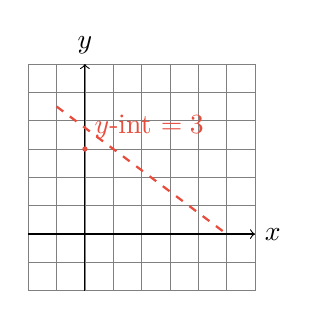
\begin{tikzpicture}[scale=0.36]
            \draw[step=1cm,gray,very thin] (-2,-2) grid (6,6);
            \draw[->] (-2,0) -- (6,0) node[right] {$x$};
            \draw[->] (0,-2) -- (0,6) node[above] {$y$};
            % Dotted boundary line
            \draw[accent,dashed,thick] (-1,4.5) -- (5, -6/2 + 3);
            % y-intercept
            \filldraw[accent] (0,3) circle (2pt);
            \node[above right,accent] at (0,3) {$y$-int $=3$};
        \end{tikzpicture}
        \end{center}
    \end{tcolorbox}
\end{frame}

% Example: Graph 3x + 2y > 6 (Step 3)
\begin{frame}{Example: Graph $3x + 2y > 6$}
    \begin{tcolorbox}[colback=secondary!10,colframe=primary,title=Step 3: Test Point]
        \footnotesize
        Use $(0,0)$ as a test point:
        \[
            3(0) + 2(0) > 6 \\
            0 > 6 \quad \textcolor{accent}{\text{False}}
        \]
        So, shade the side \textbf{not} containing $(0,0)$.
    \end{tcolorbox}
\end{frame}

% Example: Graph 3x + 2y > 6 (Step 4)
\begin{frame}{Example: Graph $3x + 2y > 6$}
    \begin{tcolorbox}[colback=secondary!10,colframe=primary,title=Step 4: Shading Solution Region]
        \footnotesize
        \begin{center}
        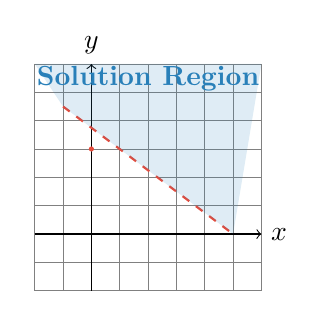
\begin{tikzpicture}[scale=0.36]
            \draw[step=1cm,gray,very thin] (-2,-2) grid (6,6);
            \draw[->] (-2,0) -- (6,0) node[right] {$x$};
            \draw[->] (0,-2) -- (0,6) node[above] {$y$};
            % Dotted boundary line
            \draw[accent,dashed,thick] (-1,4.5) -- (5, -6/2 + 3);
            % y-intercept
            \filldraw[accent] (0,3) circle (2pt);
            % Shaded region (above the line)
            \fill[primary,opacity=0.15] (-2,6) -- (6,6) -- (5, -6/2 + 3) -- (-1,4.5) -- cycle;
            \node at (2,5.5) {\textcolor{primary}{\textbf{Solution Region}}};
        \end{tikzpicture}
        \end{center}
    \end{tcolorbox}
\end{frame}

% Practice Problem
\begin{frame}{Practice: Graphing Linear Inequality}
    \begin{tcolorbox}[colback=lightgray,colframe=accent,title=Practice]
        \footnotesize
        Graph the solution set for $y \leq \frac{1}{2}x - 2$.
        \begin{itemize}
            \item Identify the boundary line and whether it is solid or dotted.
            \item Pick a test point and determine which side to shade.
        \end{itemize}
    \end{tcolorbox}
\end{frame}

% Graphing Systems of Linear Inequalities
\begin{frame}{Graphing Systems of Linear Inequalities}
    \begin{tcolorbox}[colback=lightgray,colframe=primary,title=Systems of Linear Inequalities]
        \footnotesize
        \begin{itemize}
            \item If you have two or more equations in a system of inequalities:
            \item Graph each inequality separately
            \item Shade the common area of all the inequalities involved
            \item The solution will be the common area
            \item If asked to find the area of the common shaded zone, use area formulas:
        \end{itemize}
    \end{tcolorbox}
    \vspace{0.5em}
    \textbf{Area of a Triangle:}
    \[
        A = \frac{b \times h}{2}
    \]
    \begin{center}
    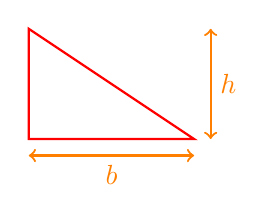
\begin{tikzpicture}[scale=0.7]
        \draw[thick,red] (0,0) -- (3,0) -- (0,2) -- cycle;
        \draw[<->,orange,thick] (0,-0.3) -- (3,-0.3);
        \node[below,orange] at (1.5,-0.3) {$b$};
        \draw[<->,orange,thick] (3.3,0) -- (3.3,2);
        \node[right,orange] at (3.3,1) {$h$};
    \end{tikzpicture}
    \end{center}
\end{frame}

% Example: Graph the system and find the area
\begin{frame}{Example: Graph the System and Find the Area}
    \begin{columns}
        \column{0.45\textwidth}
        \footnotesize
        \textbf{System:}
        \begin{align*}
            x &> 2 \\
            y &> 1 \\
            x + y &\leq 10
        \end{align*}
        \textcolor{accent}{BASE:} $=9-2=7$\\
        \textcolor{accent}{HEIGHT:} $=8-1=7$\\
        $A = \frac{7 \times 7}{2} = 24.5$ units$^2$
        \column{0.55\textwidth}
        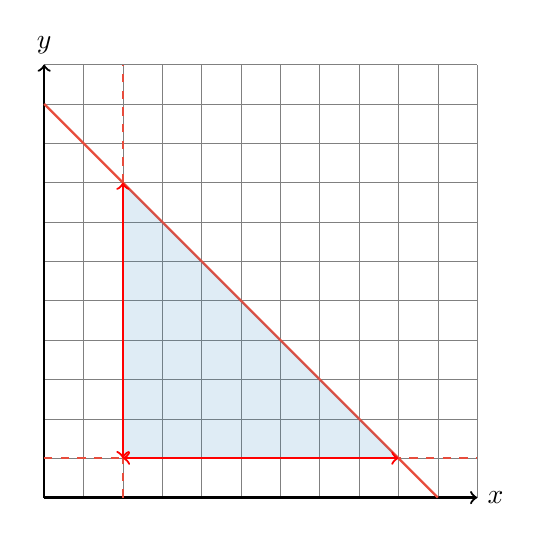
\begin{tikzpicture}[scale=0.5]
            \draw[step=1cm,gray,very thin] (0,0) grid (11,11);
            \draw[->,thick] (0,0) -- (11,0) node[right] {$x$};
            \draw[->,thick] (0,0) -- (0,11) node[above] {$y$};
            % x=2 vertical
            \draw[accent,thick,dashed] (2,0) -- (2,11);
            % y=1 horizontal
            \draw[accent,thick,dashed] (0,1) -- (11,1);
            % x+y=10
            \draw[accent,thick] (0,10) -- (10,0);
            % Shaded triangle
            \fill[primary,opacity=0.15] (2,1) -- (2,8) -- (9,1) -- cycle;
            % Base and height arrows
            \draw[red,<->,thick] (2,1) -- (9,1);
            \draw[red,<->,thick] (2,1) -- (2,8);
        \end{tikzpicture}
    \end{columns}
\end{frame}

% Example: Write the system for shaded region
\begin{frame}{Example: Write the System of Inequalities for the Shaded Region}
    \begin{columns}
        \column{0.5\textwidth}
        \footnotesize
        Pick a point in the shaded region (e.g., $(4,0)$).\\
        Use the point to determine the inequality sign.\\
        \textcolor{accent}{Dotted line:} $3y > -x$\\
        \textcolor{primary}{Solid line:} $x \leq 6$, $3y \leq x$
        \column{0.5\textwidth}
        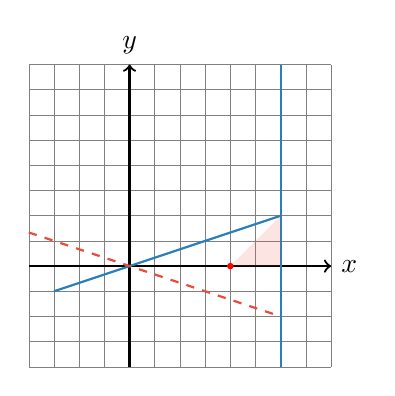
\begin{tikzpicture}[scale=0.32]
            \draw[step=1cm,gray,very thin] (-4,-4) grid (8,8);
            \draw[->,thick] (-4,0) -- (8,0) node[right] {$x$};
            \draw[->,thick] (0,-4) -- (0,8) node[above] {$y$};
            % x=6 vertical
            \draw[primary,thick] (6,-4) -- (6,8);
            % 3y=x
            \draw[primary,thick] (-3,-1) -- (6,2);
            % 3y=-x
            \draw[accent,thick,dashed] (-4,4/3) -- (6,-2);
            % Shaded triangle
            \fill[accent,opacity=0.15] (4,0) -- (6,2) -- (6,0) -- cycle;
            % Test point
            \filldraw[red] (4,0) circle (3pt);
        \end{tikzpicture}
    \end{columns}
\end{frame}

% Problems Involving Linear Inequalities
\begin{frame}{Problems Involving Linear Inequalities}
    \begin{tcolorbox}[colback=lightgray,colframe=primary,title=Translating Words to Inequalities]
        \footnotesize
        \begin{itemize}
            \item Two numbers add \textit{up to} 100: $x + y \leq 100$
            \item The sum is \textit{at least} 99: $x + y \geq 99$
            \item The sum is \textit{more than} 50: $x + y > 50$
            \item Jack's age is less than 35: $x < 35$
            \item Some variables cannot be negative: $t > 0$ (time, age, quantity)
        \end{itemize}
    \end{tcolorbox}
\end{frame}

% Application Example: Work Hours
\begin{frame}{Application Example: Work Hours}
    \begin{columns}
        \column{0.55\textwidth}
        \footnotesize
        John has 2 jobs: a stock broker for BMO and a financial planner for London Life. He works up to 55 hours a week.\\
        Let $x$ be the hours at BMO, $y$ at London Life.\\
        \begin{align*}
            x + y &\leq 55 \\
            x &\geq 0 \\
            y &\geq 0
        \end{align*}
        Graph each equation separately. The solution is the common area.
        \column{0.45\textwidth}
        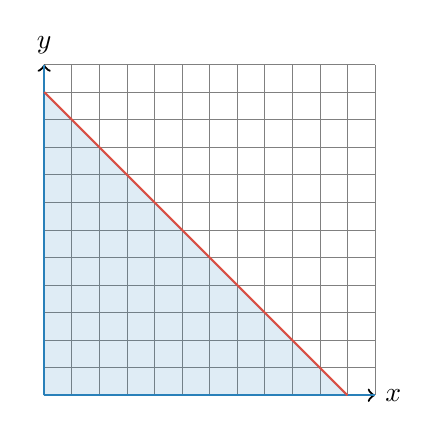
\begin{tikzpicture}[scale=0.07]
            \draw[step=5cm,gray,very thin] (0,0) grid (60,60);
            \draw[->,thick] (0,0) -- (60,0) node[right] {$x$};
            \draw[->,thick] (0,0) -- (0,60) node[above] {$y$};
            % x=0
            \draw[primary,thick] (0,0) -- (0,60);
            % y=0
            \draw[primary,thick] (0,0) -- (60,0);
            % x+y=55
            \draw[accent,thick] (0,55) -- (55,0);
            % Shaded region
            \fill[primary,opacity=0.15] (0,0) -- (0,55) -- (55,0) -- cycle;
        \end{tikzpicture}
    \end{columns}
\end{frame}

% Summary Slide
\begin{frame}{Summary: Graphing Linear Inequalities}
    \begin{tcolorbox}[colback=lightgray,colframe=primary,title=Key Points]
        \footnotesize
        \begin{itemize}
            \item \textcolor{accent}{Graph the boundary line} (solid for $\leq, \geq$; dotted for $<, >$)
            \item \textcolor{accent}{Pick a test point} (often $(0,0)$)
            \item \textcolor{accent}{Shade the region} where the test point makes the inequality true
            \item \textcolor{accent}{The shaded area is the solution set}
        \end{itemize}
    \end{tcolorbox}
\end{frame}

% Practice Problems Section
\begin{frame}{Practice Problem 1}
    \begin{tcolorbox}[colback=lightgray,colframe=accent,title=Practice 1]
        \footnotesize
        Graph the solution set for $2x - y < 4$.
    \end{tcolorbox}
\end{frame}

\begin{frame}{Practice 1: Blank Grid}
    \begin{center}
    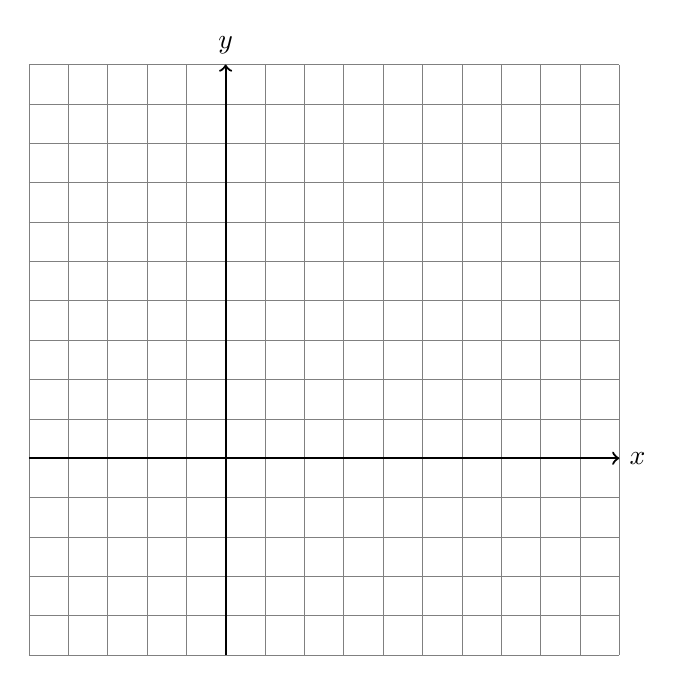
\begin{tikzpicture}[scale=0.5]
        \draw[step=1cm,gray,very thin] (-5,-5) grid (10,10);
        \draw[->,thick] (-5,0) -- (10,0) node[right] {$x$};
        \draw[->,thick] (0,-5) -- (0,10) node[above] {$y$};
    \end{tikzpicture}
    \end{center}
\end{frame}

\begin{frame}{Practice Problem 2}
    \begin{tcolorbox}[colback=lightgray,colframe=accent,title=Practice 2]
        \footnotesize
        Graph the solution set for the system:
        \begin{align*}
            x + y &\geq 2 \\
            y &< 3x - 1
        \end{align*}
    \end{tcolorbox}
\end{frame}

\begin{frame}{Practice 2: Blank Grid}
    \begin{center}
    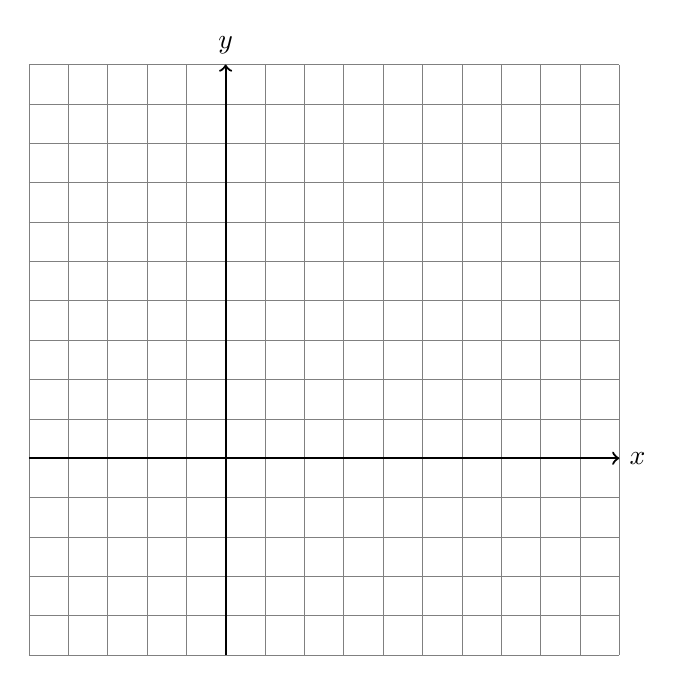
\begin{tikzpicture}[scale=0.5]
        \draw[step=1cm,gray,very thin] (-5,-5) grid (10,10);
        \draw[->,thick] (-5,0) -- (10,0) node[right] {$x$};
        \draw[->,thick] (0,-5) -- (0,10) node[above] {$y$};
    \end{tikzpicture}
    \end{center}
\end{frame}

\begin{frame}{Practice Problem 3}
    \begin{tcolorbox}[colback=lightgray,colframe=accent,title=Practice 3]
        \footnotesize
        A company can produce up to 100 units of product A and B combined. At least 30 units of A and at least 20 units of B must be produced.\\
        Write and graph the system of inequalities for the feasible region.
    \end{tcolorbox}
\end{frame}

\begin{frame}{Practice 3: Blank Grid}
    \begin{center}
    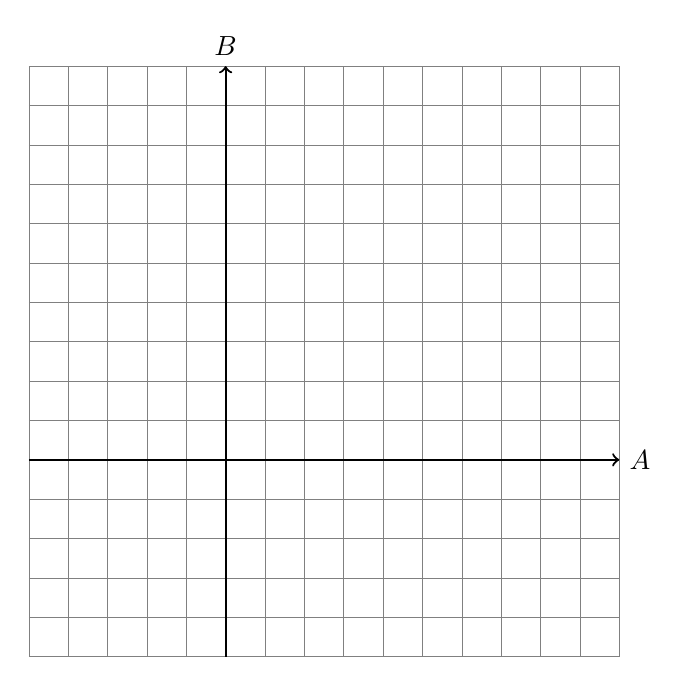
\begin{tikzpicture}[scale=0.5]
        \draw[step=1cm,gray,very thin] (-5,-5) grid (10,10);
        \draw[->,thick] (-5,0) -- (10,0) node[right] {$A$};
        \draw[->,thick] (0,-5) -- (0,10) node[above] {$B$};
    \end{tikzpicture}
    \end{center}
\end{frame}

\end{document} 